\documentclass[a4paper,12pt]{article}
\usepackage[a4paper,top=3cm,bottom=2cm,left=3cm,right=3cm,marginparwidth=1.75cm]{geometry}
\usepackage[brazil]{babel}
\usepackage[T1]{fontenc}
\usepackage[utf8]{inputenc}
\usepackage{amsmath}
\usepackage{MnSymbol}
\usepackage{wasysym}
\usepackage{hyperref}
\usepackage{color}
\definecolor{Blue}{rgb}{0,0,0.9}
\definecolor{Red}{rgb}{0.9,0,0}
\usepackage{esvect}
\usepackage{graphicx}
\usepackage{float}
\usepackage{indentfirst}
\usepackage{caption}
\usepackage{blkarray}
\newcommand\Mark[1]{\textsuperscript#1}
\usepackage{pgfplots}
\usepackage{amsfonts}
\title{Relatório de Laboratório 2}
\author{Guilherme Philippi, Carlos Eduardo dos Santos Junior}
\begin{document}
\maketitle
\tableofcontents

\section{Introdução}
Este relatório tem como objetivo apresentar soluções de sistemas a eventos discretos, usando como ferramenta de modelagem as \textit{redes de Petri}. Seguiremos a definição adotada por \cite{cardoso1997redes}, onde apresenta-se as redes de petri a partir de um modelo formal, motivado por representações em grafos de dois tipos disjuntos de nós com um comportamento dinâmico, munido de um conjunto de regras sob a forma \textit{condição} $\longrightarrow$ \textit{ação}.

Utilizou-se o software PIPE (Platform Independent Petri net Editor) \cite{dias2007ferramentas} para modelar e simular as soluções propostas, assim como segue na próxima seção.

\section{Desenvolvimento}
\subsection{Linha Industrial de Manufatura}

O primeiro problema abordado por este documento cerne sobre a modelagem, usando redes de Petri, de uma linha de manufatura com retrabalho de peças rejeitadas em fim de linha. Algumas características particulares desta linha de montagem foram especificadas, são elas:
\begin{itemize}
	\item A linha possui uma máquina $M_1$, uma máquina $M_2$ e um equipamento de aferição $A$ (que verifica a qualidade da peça processada). Cada um desses equipamentos pode processar apenas $1$ peça por vez;
	\item A máquina $M_1$ possui um \textit{buffer} de entrada $B_1$ (inicialmente com $50$ peças);
	\item A conexão entre as máquinas $M_1$ e $M_2$ ocorre através de um \textit{buffer} $B_2$ (com limite de $5$ peças);
	\item Após a peça ser processada pela máquina $M_2$, a mesma é transferida diretamente para o equipamento de aferição;
	\item Caso a peça seja aprovada, ela é envida para o estoque $E_1$. Caso seja rejeitada deve ser enviada para retrabalho. 
\end{itemize}

Seguindo essas características, modelou-se, com auxílio do software PIPE, a rede de Petri apresentada na Figura ~\ref{fig:manu}.

\begin{figure}[H]
	\begin{center}
		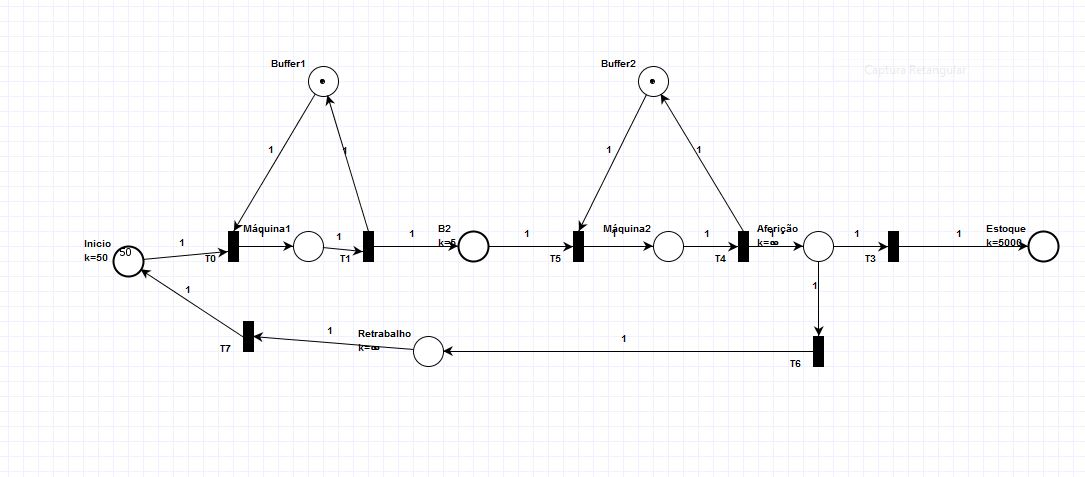
\includegraphics[width=1.05\linewidth]{manu.JPG}
	\end{center}
	\caption{Rede de Petri do sistema de manufatura}
	\label{fig:manu}
\end{figure}

Perceba que cada uma das características acima são respeitadas na modelagem desta rede. Um comentário excepcional sobre as maquinas $M_1$ e $M_2$: Note a presença de \textit{buffers} entre as suas transições finais e iniciais. Estes garantem que não entrem mais do que uma peça por vez nas maquinas. Perceba também a presença de um acumulador $B_2$ entre as duas máquinas, este pode conter até 5 elementos saídos de $M_1$ aguardando para entrarem em $M_2$.

\subsection{Sistema Ferroviário}
Neste problema o desafio era controlar um sistema ferroviário que passava por seis estações, conforme é mostrado na Figura ~\ref{fig:tremmol}. Este problema, assim como o anterior, contém algumas características particulares que foram abordadas, são elas:
\begin{itemize}
	\item  Nenhum trem pode partir de uma estação se a via férrea que liga a estação atual com a seguinte encontra-se ocupada ou a estação seguinte encontra-se também ocupada;
	\item Considere que a estação 1 da linha férrea encontra-se ligada simultaneamente com um pátio onde os trens podem se abastecer; o pátio terá a capacidade de estacionar até 10 trens; os trens podem passar da estação 1 para o pátio a qualquer momento, porem só podem passar do pátio para a estação 1 se não houver nenhum trem na estação 1, nem houver um trem na via que liga a estação 6 com a estação 1, nem houver um trem na estação 6.
\end{itemize}

\begin{figure}[H]
	\begin{center}
		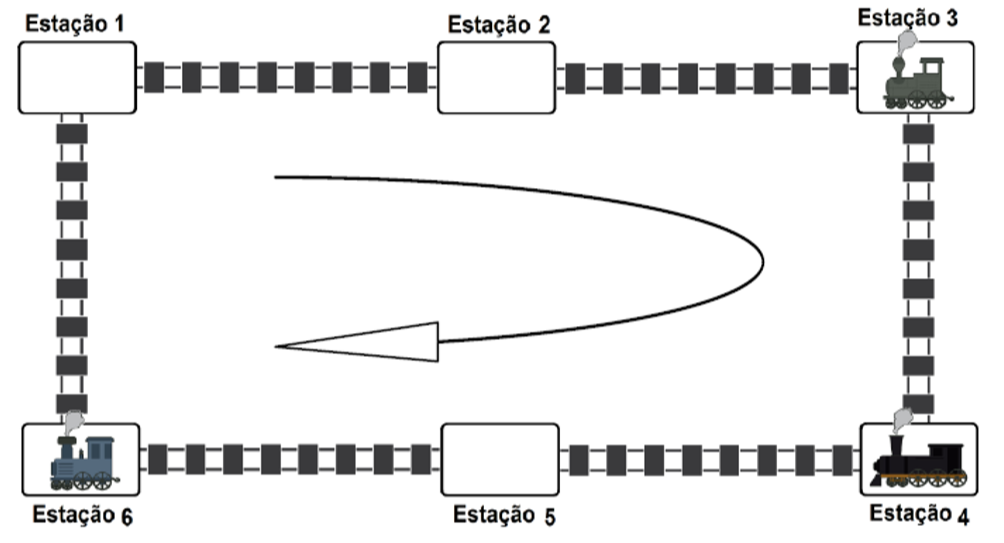
\includegraphics[width=0.8\linewidth]{tremmol.png}
	\end{center}
	\caption{Representação do sistema ferroviário}
	\label{fig:tremmol}
\end{figure}

Dada as devidas condições, também utilizando o software PIPE, modelou-se a rede de Petri apresentada na Figura ~\ref{fig:trem}.

\begin{figure}[H]
	\hspace{-0.8cm}
	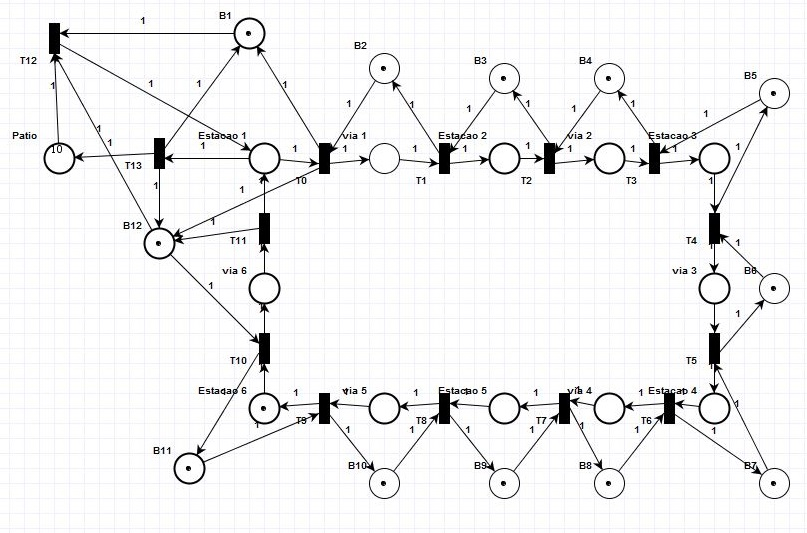
\includegraphics[width=1.1\linewidth]{trem.JPG}
	\caption{Rede de Petri que modela o sistema ferroviário}
	\label{fig:trem}
\end{figure}

Assim como no problema de manufatura, onde tínhamos que garantir que só entre uma peça por vez em cada maquina, aqui tínhamos que nos assegurar de que somente um trem utilize uma estação ou via por vez. Para isso, utilizamos a mesma solução anterior, colocou-se $buffers$ em paralelo com cada estação e via.

Pode-se perceber que, pela Figura ~\ref{fig:trem}, a complexidade estava no controle da entrada e saída de trens do pátio. Mas, como pode-se conferir, cada transição está de acordo com as especificações apresentadas.

\section{Considerações Finais}

Pode-se perceber, com o que foi apresentado, o grande poder de se trabalhar com Redes de Petri. Vale mencionar a característica abstrata que esse esquema de modelagem possui, permitindo-nos modelar sistemas dos mais variados tipos de formas incrivelmente semelhantes, isto é, simplificando-os em comportamentos comuns do tipo \textit{condição} $\longrightarrow$ \textit{ação}.

\phantomsection
\addcontentsline{toc}{section}{Referências}

\bibliographystyle{unsrt}
\bibliography{references}

\end{document}
